\chapter{\label{chp:background}Background}
In the early days of digital hardware design, gates design and layout were performed manually by hand. With the rapid growth in the numbers of transistors per digital chip design, this method quickly became too timeconsuming and thus the need for new and more automated design methods rose. \gls{rtl} design using \gls{hdl} has long been the standard in hardware design, but with the increasing demand for low power and small area in large \gls{soc} designs with multiple billion transistors, this methodology is no longer sufficient if hardware manufacturers want to hit the window of opportunity with their state-of-the-art product.

\section{\label{sec:hls}High-Level Synthesis}

\gls{hls} is not a new concept as it were introduced in research papers in the late 1970 and further researched and developed in the 1980 and early 1990s \cite{martin2009high}. The available commercial \gls{hls} tools has however not been providing the necessary performance and benefits over \gls{hdl} development for major hardware development companies to adapt this methodology until recently.
The concept of \gls{hls} is to use higher abstraction level, often a \gls{hll}, to describe the functional specification of the circuit, and then let a tool help transform this specification into hardware represented as a \gls{rtl} or \gls{hdl}-model from the given target architectural models and design constraints. The typical \gls{hls}-flow is shown in figure \ref{fig:hlsflow} and each of the transition-steps is described in the below subsections. The input libraries contain information on available hardware resources with power, area and delay models for the target architecture.

\begin{figure}[hbpt]
\centering
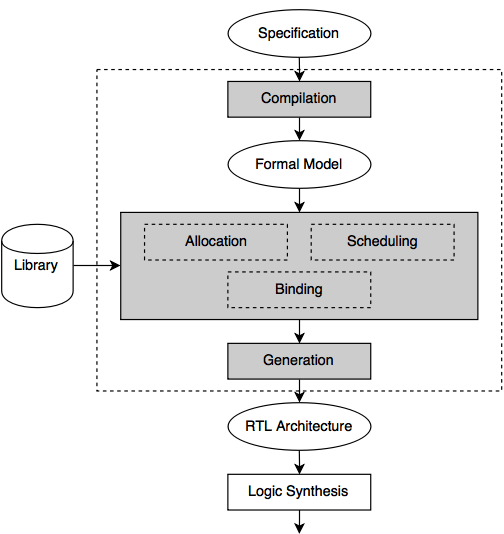
\includegraphics[width=0.6\textwidth]{../figs/HLSFlow.png}
\caption{\label{fig:hlsflow}Information flow in a typical \gls{hls} tool (source: \cite{coussy2009introduction})}
\end{figure}

\subsubsection{Compilation}

The first step of \gls{hls} is to compile the \gls{hll} into a formal model. This model can vary between different tools, and can be either a specific representation language or a graphic representation of the flow. The formal model is decided by the developers of the \gls{hls} tool. 

\subsubsection{Allocation}

Necessary hardware resources such as functional units, storage and connectivity components needs to be selected from a given \gls{rtl} component library, in order to satisfy the specification and design constraints. Some \gls{hls} tools can also add more resources in scheduling and bind task if found necessary to meet given constraints.

\subsubsection{Scheduling}
Scheduling arranges all operations in an optimized sequence so that variables are read from sources and brought to the input of the correct functional unit for execution and to the destination afterwards. The scheduler takes all dependencies into account when scheduling the operations, in order to get the most efficient result, as some operations can be executed in parallel if no dependencies exist and there is available resources. Operations can be scheduled to finish in one or take multiple clock-cycles and operations can also be chained to eliminate the need for storing the result between operations and to reduce the total number of cycles needed. 
\subsubsection{Binding}
In the binding task, all clock-cycle crossing variables, operations and transfers are bound to a free resource in the timeframe when they are scheduled. Non-overlapping or mutually exclusive variables can be bound to the the same storage unit, and operations can be bound to the best optimized functional unit if multiple alternatives are available. Each transfer from component to component, either storage or functional unit, needs to be bound to a connection unit, such as a bus or a multiplexer.
\subsubsection{RTL Generation}
The generated \gls{rtl} usually consists of two parts, a control unit and a data path unit. The control unit is often implemented as a \gls{fsm} that sets control signals to the data path, and controls the current and next-state of the system. The data path contains storage , functional and connection units. Depending on the intensiveness of the binding step, the output \gls{rtl} can be tightly or loosely bound to the available resources. If an operation is not bound to a specific unit, it is up to the following logic synthesis of the \gls{rtl} to bind the operations to available resources. The different types of \gls{rtl} output is illustrated by the following example \textit{a = b * c} executing in state \textit{n}:\\
\begin{minipage}[t][270px]{\textwidth}
\textbf{Without any binding:}%\hfill\vspace{-\baselineskip}
\begin{verbatim}
state (n): a = b * c;
go to state (n + 1);
\end{verbatim}
\textbf{With storage binding:}%\hfill\vspace{-\baselineskip}
\begin{verbatim}
state (n): S(1) = S(2) * S(3);
go to state (n + 1);
\end{verbatim}
\textbf{With functional-unit binding:}%\hfill\vspace{-\baselineskip}
\begin{verbatim}
state (n): a = MUL1 (b, c);
go to state (n + 1);
\end{verbatim}
\textbf{With storage and functional-unit binding:}%\hfill\vspace{-\baselineskip}
\begin{verbatim}
state (n): S(1)=MUL1 (S(2), S(3));
go to state (n + 1);
\end{verbatim}
\textbf{With storage, functional-unit, and connectivity binding:}%\hfill\vspace{-\baselineskip}
\begin{verbatim}
state (n): BUS1 = S(2); BUS2 = S(3);
BUS3 = MUL1 (BUS1, BUS2);
S(1) = BUS3;
go to state (n + 1);
\end{verbatim}
\end{minipage}
A loosely bound \gls{rtl} gives the synthesis the flexibility to optimize the unit binding to updates timing estimates and delays and loads given by the layout and floor-planning.
\section{LegUp}
The \gls{hls} tool used in this project is called LegUp \cite{canis2011legup}. LegUp is an open-source academic tool developed at the University of Toronto, Canada. LegUp's goal is to \textit{"allow researchers to experiment with new \gls{hls} algorithms without building a new infrastructure from scratch"} and their long-term vision is to \textit{"make \gls{fpga} programming easier for software developers"}. LegUp takes \acrshort{ansi} C as input and generates synthesizable Verilog \gls{hdl} as output. The developers of LegUp has primarily focused on support for a variety of \gls{fpga} boards from manufacturer Altera, but in the latest version (4.0), beta support for Xilinx devices and possibility to configure the tool to generate generic Verilog to target other \gls{fpga} vendors or even \gls{asic} through use of generic dividers, has been introduced. The big advantage of LegUp compared to similar, commercial tools is that it's open-source and thus can be configured to target different architectures, and the \gls{rtl} and \gls{hdl} generating part of the framework can be modified or replaced to fit the programmers needs.
Since LegUp, in it's unmodified form, targets \gls{fpga} devices, it support three different synthesis flows; pure \gls{sw}, hybrid and pure \gls{hw}. The two first synthesis types will synthesize a TigerMIPS \cite{tigmips} soft processor, which will run the whole C file in pure \gls{sw} flow and part of the C file in hybrid flow while the rest will be synthesized into hardware. The pure \gls{hw} flow will synthesise the whole C file into hardware. It's the pure \gls{hw} flow that will be the focus of this project.

\subsubsection{Producing Verilog Output}

LegUp is made up of two components; a frontend pass and a target backend pass to the \gls{llvm} compiler infrastructure. 
The information flow in LegUp, shown in figure \ref{fig:legupflow}, follows the same principle as the information flow described in section \ref{sec:hls} 
\begin{figure}[hbpt]
\centering
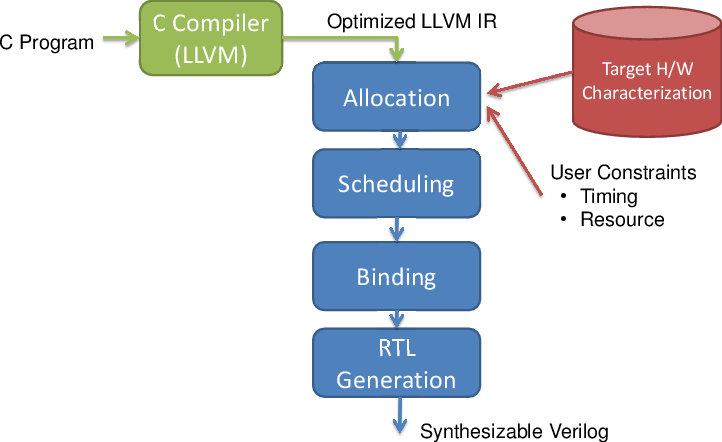
\includegraphics[width=0.6\textwidth]{../figs/LegUpFlow.png}
\caption{\label{fig:legupflow}Information flow in LegUp (source: http://legup.eecg.utoronto.ca/docs/4.0/programmermanual.html)}
\end{figure}
The LegUp \gls{llvm} frontend takes \gls{llvm} \gls{ir} compiled by clang frontend for \gls{llvm} as input and links in custom written functions like memcpy, memset and memmove, which do not exist in hardware, but that \gls{llvm} assumes exist in the C library. 
The LegUp backend pass performs allocation, scheduling and binding as described in section \ref{sec:hls}. In the next step, \gls{rtl}-module objects that represents the final hardware circuit are generated from each \gls{llvm} instruction. Ultimately, each \gls{rtl}-module is printed to a file using the corresponding Verilog code for the given \gls{hw} module.

\section{\label{sec:LLVM}LLVM}

\gls{llvm} \cite{LLVM:CGO04} is a compiler framework that was originally developed as a research infrastructure to investigate dynamic compilation techniques for static and dynamic programming languages, at the University of Illinois in 2000. It is now a open-source project with many contributors from both industry, research groups and individuals, and is widely used by for instance companies like Apple and Sony for iOS and PS4 development. \gls{llvm} support a large number of frontends for programming languages, including Clang \cite{clang} which support C, C++, Obcjective-C and Objective-C++ and is compatible with GCC. It also supports a large number of backend target architectures. Figure \ref{fig:llvmcompiler} shows how different source languages can be input to the \gls{llvm} compiler, which translate the source into an \gls{ir}. The \gls{ir} is then optimized using \gls{llvm}s optimizer. At this stage, different source languages can be linked together, and one can even link object files compiled using standard \gls{gcc}. The optimized \gls{ir} is then translated into the target architecture by the backend.

\begin{figure}[hbpt]
\centering
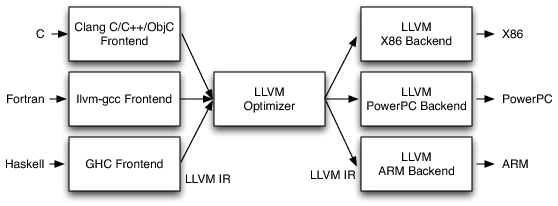
\includegraphics[width=\textwidth]{../figs/LLVMCompiler.png}
\caption{\label{fig:llvmcompiler}LLVMs three-phase compiler structure (source: http://www.aosabook.org/en/llvm.html)}
\end{figure}
\subsubsection{Intermediate Representation}

\gls{llvm} uses an human readable assembly-like, strongly typed RISC instruction set as their \gls{ir}, with support for an infinite number of temporary registers of the form \%0, \%1, etc. \gls{llvm} \gls{ir} can also output a dense bitcode format for serialization.

\section{\label{sec:powest}Power and area estimation}

In order to compare different use-cases and result generated by LegUp, the area and power-usage will be estimated. Since this is not the main objective of this project, the automated area and power estimation tool-flow created by Joar Talstad in his specialization project \cite{talstad14project} and master thesis \cite{talstad15master} will be adapted for this purpose. The tool-flow he created uses Synopsys Primetime PX for power analysis and estimation.

\section{Information and tool-flow}
LegUp utilizes Makefiles to perform the \gls{hls} flow. The power and area estimation tool-flow described in section \ref{sec:powest} also use Makefiles for its flow. It will thus be suitable to create a single Makefile that controls the information flow from the input of a C file to the output of Verilog files along with scorefiles on the area and power estimates. 